\documentclass[letterpaper, 11pt]{extarticle}
% \usepackage{fontspec}

% ==================================================

% document parameters
% \usepackage[spanish, mexico, es-lcroman]{babel}
\usepackage[english]{babel}
\usepackage[margin = 1in]{geometry}

% ==================================================

% Packages for math
\usepackage{mathrsfs}
\usepackage{amsfonts}
\usepackage{amsmath}
\usepackage{amsthm}
\usepackage{amssymb}
\usepackage{physics}
\usepackage{dsfont}
\usepackage{esint}

% ==================================================

% Packages for writing
\usepackage{enumerate}
\usepackage[shortlabels]{enumitem}
\usepackage{framed}
\usepackage{csquotes}

% ==================================================

% Miscellaneous packages
\usepackage{float}
\usepackage{tabularx}
\usepackage{xcolor}
\usepackage{multicol}
\usepackage{subcaption}
\usepackage{caption}
\captionsetup{format = hang, margin = 10pt, font = small, labelfont = bf}

% Citation
\usepackage[round, authoryear]{natbib}

% Hyperlinks setup
\usepackage{hyperref}
\definecolor{links}{rgb}{0.36,0.54,0.66}
\hypersetup{
   colorlinks = true,
    linkcolor = black,
     urlcolor = blue,
    citecolor = blue,
    filecolor = blue,
    pdfauthor = {Author},
     pdftitle = {Title},
   pdfsubject = {subject},
  pdfkeywords = {one, two},
  pdfproducer = {LaTeX},
   pdfcreator = {pdfLaTeX},
   }
\usepackage{titlesec}
\usepackage[many]{tcolorbox}

% Adjust spacing after the chapter title
\titlespacing*{\chapter}{0cm}{-2.0cm}{0.50cm}
\titlespacing*{\section}{0cm}{0.50cm}{0.25cm}

% Indent 
\setlength{\parindent}{0pt}
\setlength{\parskip}{1ex}

% --- Theorems, lemma, corollary, postulate, definition ---
% \numberwithin{equation}{section}

\newtcbtheorem[]{problem}{}%
    {enhanced,
    colback = black!5, %white,
    colbacktitle = black!5,
    coltitle = black,
    boxrule = 0pt,
    frame hidden,
    borderline west = {0.5mm}{0.0mm}{black},
    fonttitle = \bfseries,
    breakable,
    before skip = 3ex,
    after skip = 3ex
}{problem}

\tcbuselibrary{skins, breakable}

% --- You can define your own color box. Just copy the previous \newtcbtheorm definition and use the colors of yout liking and the title you want to use.
% --- Basic commands ---
%   Euler's constant
\newcommand{\eu}{\mathrm{e}}

%   Imaginary unit
\newcommand{\im}{\mathrm{i}}

%   Sexagesimal degree symbol
\newcommand{\grado}{\,^{\circ}}

% --- Comandos para álgebra lineal ---
% Matrix transpose
\newcommand{\transpose}[1]{{#1}^{\mathsf{T}}}

%%% Comandos para cálculo
%   Definite integral from -\infty to +\infty
\newcommand{\Int}{\int\limits_{-\infty}^{\infty}}

%   Indefinite integral
\newcommand{\rint}[2]{\int{#1}\dd{#2}}

%  Definite integral
\newcommand{\Rint}[4]{\int\limits_{#1}^{#2}{#3}\dd{#4}}

%   Dot product symbol (use the command \bigcdot)
\makeatletter
\newcommand*\bigcdot{\mathpalette\bigcdot@{.5}}
\newcommand*\bigcdot@[2]{\mathbin{\vcenter{\hbox{\scalebox{#2}{$\m@th#1\bullet$}}}}}
\makeatother

%   Hamiltonian
\newcommand{\Ham}{\hat{\mathcal{H}}}

%   Trace
\renewcommand{\Tr}{\mathrm{Tr}}

% Christoffel symbol of the second kind
\newcommand{\christoffelsecond}[4]{\dfrac{1}{2}g^{#3 #4}(\partial_{#1} g_{#2 #4} + \partial_{#2} g_{#1 #4} - \partial_{#4} g_{#1 #2})}

% Riemann curvature tensor
\newcommand{\riemanncurvature}[5]{\partial_{#3} \Gamma_{#4 #2}^{#1} - \partial_{#4} \Gamma_{#3 #2}^{#1} + \Gamma_{#3 #5}^{#1} \Gamma_{#4 #2}^{#5} - \Gamma_{#4 #5}^{#1} \Gamma_{#3 #2}^{#5}}

% Covariant Riemann curvature tensor
\newcommand{\covariantriemanncurvature}[5]{g_{#1 #5} R^{#5}{}_{#2 #3 #4}}

% Ricci tensor
\newcommand{\riccitensor}[5]{g_{#1 #5} R^{#5}{}_{#2 #3 #4}}

\usepackage{placeins}
\usepackage{listings}
\usepackage{xcolor}

% Define a custom style for VHDL
\lstdefinelanguage{VHDL}{
    keywords=[1]{library, use, entity, is, port, in, out, architecture, of, begin, end, process},
    keywords=[2]{signal, STD_LOGIC, STD_LOGIC_VECTOR},
    keywordstyle=[1]\color{blue}\bfseries,
    keywordstyle=[2]\color{teal}\bfseries,
    sensitive=true,
    morecomment=[l]--,
    morestring=[b]"
}

\lstset{
    language=VHDL,
    basicstyle=\ttfamily\footnotesize,
    numbers=left,
    numberstyle=\tiny\color{gray},
    keywordstyle=\color{blue},
    commentstyle=\color{green!60!black},
    stringstyle=\color{orange},
    breaklines=true,
    showstringspaces=false,
    tabsize=2,
    xleftmargin=2em
}

\begin{document}

\begin{Large}
    \textsf{\textbf{Moltiplicatore Binario}}\\
\end{Large}
\textbf{Relazione di progetto}

\vspace{1ex}

\textsf{\textbf{Studenti:}} \\
\text{Frega Umberto 239527}, \href{frgmrt04a05l353d@studenti.unical.it}{\texttt{frgmrt04a05l353d@studenti.unical.it}};\\
\text{Napoli Leonardo 234364}, \href{npllrd02s30d086@studenti.unical.it} {\texttt{npllrd02s30d086@studenti.unical.it}};

\href{https://github.com/Zi0LEO/elettronica_digitale}{\texttt{Codice Sorgente}}


\vspace{2ex}

Il progetto assegnato consiste nel progettare ed implementare una moltiplicatore carta e penna.
Per la progettazione del sistema si è deciso di utilizzare un pattern comportamentale, andando quindi a definire il comportamento del sistema in base a determinate condizioni, oltretutto si è optato per l'utilizzo del tipo \textit{STD\_LOGIC} e quindi \textit{STD\_LOGIC\_VECTOR} per una maggiore flessibilità e maggiori funzionalità.

Il primo passo della progettazione è stato definire il carry-save-adder, e di conseguenza l'adder tree a 5 livelli.
\section{Carry-Save-Adder}
\subsection{Implementazione}
La componente di base del sistema è un carry-save-adder.
Di seguito riportiamo il codice per implementarlo.

\begin{problem}{Codice adder}{problem-label}
\begin{lstlisting}[language=VHDL]
library IEEE;
use IEEE.STD_LOGIC_1164.ALL;
    
entity carry_save_adder is
 generic (nbit_csa : INTEGER := 16);
     Port ( 
       A,B,C: in STD_LOGIC_VECTOR (nbit_csa-1 downto 0);
       sum: out STD_LOGIC_VECTOR (nbit_csa downto 0);
       carry: out STD_LOGIC_VECTOR (nbit_csa downto 0));
end carry_save_adder;
    
architecture Behavioral of carry_save_adder is

    signal sub_sum,sub_carry : STD_LOGIC_VECTOR (nbit_csa-1 downto 0);
        
  begin
    sub_sum  <= A xor B xor C;
    sub_carry <= (A and B) or (B and C) or (C and A);
    carry <= sub_carry & '0';
    sum <= '0' & sub_sum;
    
end Behavioral;
\end{lstlisting}
\end{problem}

\section{Adder-tree}
\subsection{Implementazione}
L'adder tree presenta 5 livelli, a partire dal livello 0 fino al livello 4, ogni adder presenta 3 input e 2 output, fino all'adder finale, che si presenta come un adder generico ad 2 input ed 1 output.

\begin{problem}{Codice Adder Tree}{}
\begin{lstlisting}[language=VHDL]
library IEEE;
use IEEE.STD_LOGIC_1164.ALL;
use work.AdderTree_Types.all;

entity adder_tree is
    generic (nbit : INTEGER := 32);
    
    port ( p: MAT;
            ris : out STD_LOGIC_VECTOR(nbit-1 downto 0));
    
end adder_tree;

architecture Behavioral of adder_tree is

    component carry_save_adder is 
        generic (nbit_csa : INTEGER := 31);
         Port ( 
           A,B,C: in STD_LOGIC_VECTOR (nbit_csa-1 downto 0);
           sum: out STD_LOGIC_VECTOR (nbit_csa downto 0);
           carry: out STD_LOGIC_VECTOR (nbit_csa downto 0));
     end component;     
   
     component generic_adder is 
        generic (bit_number : INTEGER := 32);
        Port ( A_adder,B_adder: in STD_LOGIC_VECTOR (bit_number-2 downto 0);
         sum_adder : out STD_LOGIC_VECTOR (bit_number-1 downto 0));
     end component;
    
    type MAT_0 is array ( 4 downto 0 ) of STD_LOGIC_VECTOR(nbit-2 downto 0);
     signal sum_0 : MAT_0;
     signal carry_0: MAT_0;
    type MAT_1 is array ( 2 downto 0 ) of STD_LOGIC_VECTOR(nbit-2 downto 0);
     signal sum_1 : MAT_1;
     signal carry_1: MAT_1;
    type MAT_2 is array ( 1 downto 0 ) of STD_LOGIC_VECTOR(nbit-2 downto 0);
     signal sum_2 : MAT_2;
     signal carry_2: MAT_2;
     
    type MAT_3 is array ( 1 downto 0 ) of STD_LOGIC_VECTOR(nbit-2 downto 0);
     signal sum_3 : MAT_3;
     signal carry_3: MAT_3;
     
     signal sum_4 :STD_LOGIC_VECTOR ( nbit-2 downto 0);
     signal carry_4: STD_LOGIC_VECTOR ( nbit-2 downto 0);
     
     signal carry_final : STD_LOGIC_VECTOR (nbit-2 downto 0);
     signal sum_final: STD_LOGIC_VECTOR (nbit-2 downto 0);
     
     signal garbage: STD_LOGIC;
     
begin 
    --lvl_0
    level0_adder: for i in 0 to (nbit/2)/3 - 1 generate
      adder0: carry_save_adder 
      PORT MAP(p(i*3), p(i*3+1),p(i*3+2), sum(30 downto 0) => sum_0(i), sum(31) => garbage, carry(30 downto 0) => carry_0(i), carry(31) => garbage);
    end generate;
    
    --lvl_1
    adder10: carry_save_adder PORT MAP(sum_0(0), sum_0(1), sum_0(2),sum(30 downto 0) => sum_1(0), sum(31) => garbage, carry(30 downto 0) => carry_1(0), carry(31) => garbage);
    adder11: carry_save_adder PORT MAP(carry_0(0), carry_0(1), carry_0(2),sum(30 downto 0) => sum_1(1), sum(31) => garbage, carry(30 downto 0) => carry_1(1), carry(31) => garbage);
    adder12: carry_save_adder PORT MAP(sum_0(3), carry_0(3), sum_0(4),sum(30 downto 0) => sum_1(2), sum(31) => garbage, carry(30 downto 0) => carry_1(2), carry(31) => garbage);
      
    --lvl_2 
    adder20: carry_save_adder PORT MAP(sum_1(0), sum_1(1), sum_1(2),sum(30 downto 0) => sum_2(0), sum(31) => garbage, carry(30 downto 0) => carry_2(0), carry(31) => garbage);
    adder21: carry_save_adder PORT MAP(carry_1(0), carry_1(1), carry_1(2),sum(30 downto 0) => sum_2(1), sum(31) => garbage, carry(30 downto 0) => carry_2(1), carry(31) => garbage);
    
    --lvl_3 
    adder30: carry_save_adder PORT MAP(sum_2(0), sum_2(1), carry_2(0),sum(30 downto 0) => sum_3(0), sum(31) => garbage, carry(30 downto 0) => carry_3(0), carry(31) => garbage);
    adder31: carry_save_adder PORT MAP(carry_2(0), carry_0(4), p(15),sum(30 downto 0) => sum_3(1), sum(31) => garbage, carry(30 downto 0) => carry_3(1), carry(31) => garbage);

     --lvl_4 
    adder40: carry_save_adder PORT MAP(sum_3(0), sum_3(1), carry_3(0),sum(30 downto 0) => sum_4, sum(31) => garbage, carry(30 downto 0) => carry_4, carry(31) => garbage);
 
     -- lvl_5
    adder50: carry_save_adder PORT MAP(sum_4, carry_4, carry_3(1),sum(30 downto 0) => sum_final, sum(31) => garbage, carry(30 downto 0) => carry_final, carry(31) => garbage);

    final_adder: generic_adder
      PORT MAP (sum_final, carry_final, ris);
end Behavioral;

\end{lstlisting}
\end{problem}

Possiamo trovare la schematica risultante nella \textit{Figure 1}
\begin{figure}[ht]
    \centering
    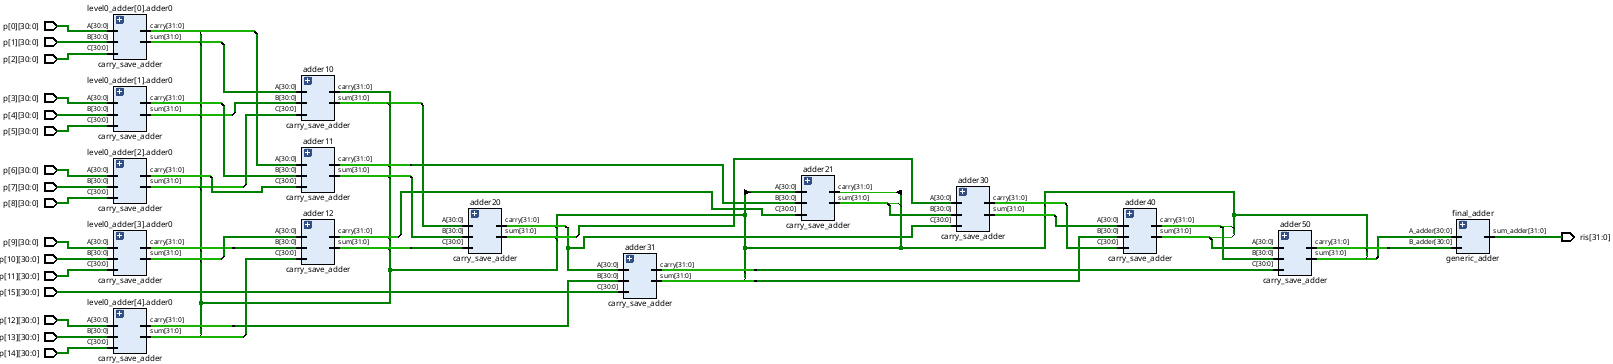
\includegraphics[width=15cm]{assets/schematics1.png}
    \caption{Circuito Logico dell'adder tree}
\end{figure}

\clearpage
\section{Moltiplicatore Binario}

\subsection{Implementazione}
Riportiamo di seguito il codice utilizzato per il moltiplicatore binario.

\begin{problem}{Codice adder}{problem-label}
\begin{lstlisting}[language=VHDL]
library IEEE;
use IEEE.STD_LOGIC_1164.ALL;
use IEEE.NUMERIC_STD.ALL;
use work.AdderTree_Types.all;

entity moltiplicatore is
    generic (nbit : INTEGER := 16);
    Port ( 
      A,B : in STD_LOGIC_VECTOR (nbit-1 downto 0); --16bit
      clk: in STD_LOGIC;
      prod : out STD_LOGIC_VECTOR ((nbit*2)-1 downto 0)); --32bit
end moltiplicatore;

architecture Behavioral of moltiplicatore is
  component adder_tree is
    port ( p: MAT;
            ris : out STD_LOGIC_VECTOR(nbit*2-1 downto 0));
  end component;
  
  signal p: MAT;
  signal IA, IB: STD_LOGIC_VECTOR(nbit-1 downto 0);
  signal Oprod: STD_LOGIC_VECTOR((nbit*2)-1 downto 0);
  signal zeros: STD_LOGIC_VECTOR(nbit-1 downto 0);
  begin     
  
  partial_products:process(clk)
  variable bucket: STD_LOGIC_VECTOR((nbit*2)-2 downto 0);

  begin
   
    if rising_edge(clk) then
      IA <= A;
      IB <= B;
      zeros <= (others => '0');
      prod <= Oprod;
      
      outer: for i in nbit-1 downto 0 loop
        inner: for j in nbit-1 downto 0 loop
          bucket(j) := IA(i) and IB(j);
        end loop inner;
        
      bucket := zeros(nbit-2 downto 0) & bucket (nbit-1 downto 0);
      p(i) <= STD_LOGIC_VECTOR(shift_left(UNSIGNED(bucket),i));
      
      end loop outer;
     end if;
  end process;
  
  adder:adder_tree
    PORT MAP(p, Oprod);
    
end Behavioral;
\end{lstlisting}
\end{problem}

Non riportiamo la schematica a causa delle grandi dimensioni.

\subsection{Simulazione}
Nella testbench abbiamo inserito 4 test che cercano di racchiudere i casi possibili.

\begin{problem}{Codice adder}{problem-label}
\begin{lstlisting}[language=VHDL]
library IEEE;
use IEEE.STD_LOGIC_1164.ALL;
use IEEE.NUMERIC_STD.ALL;

entity testench_moltiplicatore is
 generic (nbit : INTEGER := 16);
end testench_moltiplicatore;

architecture Behavioral of testench_moltiplicatore is
  component moltiplicatore is
    port ( 
      A : in STD_LOGIC_VECTOR (nbit-1 downto 0); --16bit
      B : in STD_LOGIC_VECTOR (nbit-1 downto 0); --16bit
      clk: in STD_LOGIC;
      prod : out STD_LOGIC_VECTOR ((nbit*2)-1 downto 0)); --32bit
  end component;
  
  signal IA, IB : STD_LOGIC_VECTOR (15 downto 0);
  signal Oprod : STD_LOGIC_VECTOR(31 downto 0);
  signal Iclk: STD_LOGIC := '0';
  constant Tclk : time := 10ns;
  
begin
  CUT: moltiplicatore 
    PORT MAP(A => IA, B => IB, clk => Iclk, prod => Oprod);

  process
  begin
    
    -- Test 1: A = 1, B = 1
    IA <= std_logic_vector(to_unsigned(1, IA'length)); -- Assign 0 directly
    IB <= std_logic_vector(to_unsigned(1, IB'length));
    wait for Tclk;
 
    -- Test 2: A = 0, B = 10000
    IA <= std_logic_vector(to_unsigned(0, IA'length));
    IB <= std_logic_vector(to_unsigned(10000, IB'length));
    wait for Tclk;
   
    -- Test 3: A = 100, B = 25
    IA <= std_logic_vector(to_unsigned(100, IA'length));
    IB <= std_logic_vector(to_unsigned(25, IB'length));
    wait for Tclk;    
    
    -- Test 4: A = 1, B = 15
    IA <= std_logic_vector(to_unsigned(1, IA'length));
    IB <= std_logic_vector(to_unsigned(15, IB'length));
    wait for Tclk;
  end process;
  
  process
  begin
    wait for Tclk/2;
    Iclk <= not Iclk;
  end process;
end Behavioral;
\end{lstlisting}
\end{problem}

Il risultato nelle simulazioni post-implementation è questo:
\begin{figure}[ht]
  \centering
  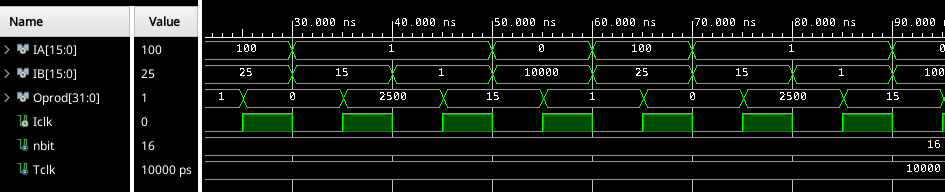
\includegraphics[width=1\textwidth]{assets/simulation.png}
  \caption{Simulazione post-implementation}
\end{figure}
Come possiamo notare dalla figura, è stato inserito anche un segnale di clock, la time constraint nel segnale di clock fissata a 10 ns ci permette di avere un wattaggio, e di conseguenza una temperatura accettabili.
\begin{figure}[ht]
  \centering
  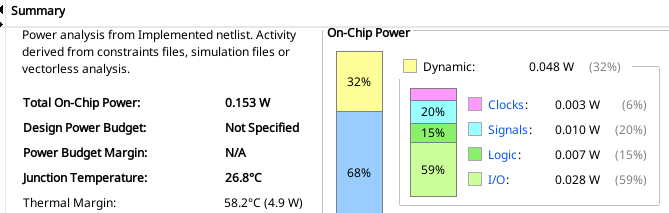
\includegraphics[width=1\textwidth]{assets/power.png}
  \caption{Post-implementation power report}
\end{figure}

\clearpage
\subsection{LUT Tables}
Dalla sintesi del circuito ci vengono restituite inoltre le LUT Tables con i relativi valori di utilizzo.

\begin{table}[ht]
      \centering
      \begin{tabular}{|c|c|c|}
        \hline
        Nome & Utilizzate \\ \hline
        BUFG & 1 \\ \hline
        LUT1 & 17 \\ \hline
        LUT2 & 16 \\ \hline
        LUT3 & 124 \\ \hline
        LUT4 & 21  \\ \hline
        LUT5 & 111 \\ \hline
        LUT6 & 161 \\ \hline
        FDRE & 288 \\ \hline
        IBUF & 33 \\ \hline
        OBUF & 32 \\ \hline
      \end{tabular}
      \caption{Numero LUT utilizzati}
\end{table}
\end{document}
